\documentclass[class=article, crop=false, 12pt]{standalone}
\usepackage[subpreambles=true]{standalone}
\usepackage{../.common/common}


\author{Tony Shing}
%\pretitle{Supplementary}

\topic{Note 04 (Math for Physics)}
\title{Matrices and System of ODEs}

\version{2025} % leave blank for omitting

\begin{document}

\maketitle

\begin{overview}
    \begin{itemize}
        \item Matrix and determinant arithmetics.
        \item Theory of system of linear equations
        \item Eigenvalue \& eigenvector
        \item Solving system of ODE - Coupled harmonic oscillators
    \end{itemize}

    \begin{center}
        \begin{minipage}{0.3\linewidth}
            \centering
            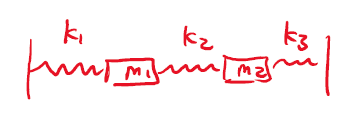
\includegraphics[width=\textwidth]{couple}
        \end{minipage}
    \end{center}

\end{overview}





% content begins here
% Section %%%%%%%%%%%%%%%%%%%%%%%%%%%%%%%%%%%%%%%%%%%%%%%%%%%%
\section{Matrices \& Determinants}

Matrix is a mathematical tool to express an array of values.
\aleq{
    \tkm{matbold}\mmat{A} = \tkbmat{
        a_{11} \& a_{12} \& a_{13} \\
        a_{21} \& a_{22} \& a_{23} \\
    }{
        \draw[<->, draw=red] (m-2-1.south west |- m.south) to ["3" ' red] (m-2-3.south east |- m.south);
        \coordinate (e) at ($(m.east) + (3ex,0)$) ;
        \draw[<->, draw=red] (m-1-3.north east -| e) to ["2" red] (m-2-3.south east -| e);
        \draw[draw=green] (m-2-3) circle (1.8ex);
    }
    \ \tkm{dim}
}
\addArrow[blue]{matbold}{(-6ex,0)}{Usually use\\bold font capital letter\\to represent matrix}{(-1ex,0.5ex)}{(-11ex,0)}
\addArrow[red]{dim}{(6ex,1ex)}{Dimension\\of this matrix\\$=2\times 3$}{(1ex,0.5ex)}{(5ex,1.5ex)}
\addArrow[green]{dim}{(5ex,-3ex)}{Each entry is called an "element"}{(-7.5ex,-2ex)}{(16ex,0)}

We call the shape ((\# of rows) $\times$ (\# of columns)) of a matrix as its \bf{dimension}. 
Depending on its shape, they may aquire special name:

\begin{center}
    \begin{minipage}[t]{0.3\textwidth}
        \centering
        \ul{Column matrix}
        \aleq{
            \bmat{
                a_1 \\ a_2 \\ \vdots \\ a_n
            }
        }
    \end{minipage}
    %
    \begin{minipage}[t]{0.3\textwidth}
        \centering
        \ul{Row matrix}
        \aleq{
            \bmat{
                a_1 & a_2 & \cdots & a_n
            }
        }
    \end{minipage}
    %
    \begin{minipage}[t]{0.3\textwidth}
        \centering
        \ul{Square matrix}\\
        (\# of rows = \# of columns)
        \aleq{
            \bmat{
                a_{11} & a_{12} & a_{13} \\
                a_{21} & a_{22} & a_{23} \\
                a_{31} & a_{32} & a_{33}
            }
        }
    \end{minipage}
\end{center}


\newpage
%%%%%%%%%%%%%%
\subsection{Matrix Arithmatics}

Matrices calculations share similar operations as calculating number, 
but with different definitions. 

\begin{enumerate}

    \item \bf{\ul{Addition / Subtraction}}
    
    Can only be carried out between matrices of the same dimension. 
    Each element is added / subtracted independently.
    \aleq{
        \mmat{A} \pm \mmat{B} = \bmat{\xmat*{a}{2}{3}} \pm \bmat{\xmat*{b}{2}{3}} 
        = \bmat{a_{11}\pm b_{11} & a_{12}\pm b_{12} & a_{13}\pm b_{13} \\
                a_{21}\pm b_{21} & a_{22}\pm b_{22} & a_{23}\pm b_{23}}
    }

    %%%
    \item \bf{\ul{Multiplication with Constants}}
    
    Multiplying a constant = Multiply every element with that constant
    \aleq{
        k\mmat{A} = k\cdot \bmat{\xmat*{a}{2}{3}} = \bmat{\xmat*{ka}{2}{3}}
    }


    %%%
    \item \bf{\ul{Transpose}}
    
    Flip the matrix diagonally. Denote using the $\intercal$ symbol.
    \aleq{
        \mmat{A} = 
        \tkbmat{
            a_{11} \& a_{12} \& a_{13} \\
            a_{21} \& a_{22} \& a_{23} \\
        }{
            \coordinate (e) at ($(m-2-3.south) + (2ex,-3ex)$);
            \draw[draw=green] (m-1-1.north west) to (e);
            \node[color=green, rotate=-90] at ($(e) - (1ex,-0.5ex)$) {$\clockwise$};
        }
        \quad \Leftrightarrow \quad 
        \mmat{A}^\intercal =
        \tkbmat{
            a_{11} \& a_{21} \\
            a_{12} \& a_{22} \\
            a_{13} \& a_{23} \\
        }{
            \coordinate (e) at ($(m-3-2.east) + (5ex,-2ex)$);
            \draw[draw=green] (m-1-1.north west) to (e);
            \node[color=green, rotate=-135] at ($(e) - (1ex,-0.5ex)$) {$\anticlockwise$};
        }
    }

    %%%
    \item \bf{\ul{Matrices Multiplication}}
    
    Given 2 matrices, one with dimension $\ul{\blue{m}\times \green{n}}$ and the other $\ul{\green{n}\times \red{p}}$,
    \aleq{
        \mmat{A} = \bmat{
            a_{11} & a_{12} & \cdots & a_{1\green{n}} \\
            a_{21} & a_{22} & \cdots & a_{2\green{n}} \\
            \vdots & \vdots & \ddots & \vdots \\
            a_{\blue{m}1} & a_{\blue{m}2} & \cdots & a_{\blue{m}\green{n}}\\
        }
        %
        \qquad , \qquad
        %
        \mmat{B} = \bmat{
            b_{11} & b_{12} & \cdots & b_{1\red{p}} \\
            b_{21} & b_{22} & \cdots & b_{2\red{p}} \\
            \vdots & \vdots & \ddots & \vdots \\
            b_{\green{n}1} & b_{\green{n}2} & \cdots & b_{\green{n}\red{p}}
        }
    }

    Their multiplication yield a product matrix of dimension $\ul{\blue{m}\times \red{p}}$. 
    \aleq{
        \mmat{C} = \tkn{mult_symb}{\cul[green]{\mmat{AB}}} = \bmat{
            c_{11} & c_{12} & \cdots & c_{1\red{p}} \\
            c_{21} & c_{22} & \cdots & c_{2\red{p}} \\
            \vdots & \vdots & \ddots & \vdots \\
            c_{\blue{m}1} & c_{\blue{m}2} & \cdots & c_{\blue{m}\red{p}}
        }
    }
    \addBentArrow[green]{mult_symb}{(-8ex,-4ex)}{We don't write $\times$ sign\\in matrix multiplication}
    {(0,-1ex)}{(-10ex,1ex)}

    The computation of each element $c$ is a sum-product of $a$ and $b$:
    \aleq{
        c_{\blue{i}\red{j}} &= \sum_{\green{k=1}}^{\green{n}} a_{\blue{i}\green{k}}b_{\green{k}\red{j}} \\
        %
        &= a_{\blue{i}\green{1}}b_{\green{1}\red{j}} + a_{\blue{i}\green{2}}b_{\green{2}\red{j}}
            + ... + a_{\blue{i}\green{n}}b_{\green{n}\red{j}}\\[1em]
        %
        %
        \tkbmat{
            \& \& \vdots \& \& \\
            \& \& \vdots \& \& \\
            \cdots \& \cdots \& c_{\blue{i}\red{j}} \& \cdots \& \cdots \\
            \& \& \vdots \& \& \\
            \& \& \vdots \& \& \\
        }{
            \draw[->,draw=blue] ($(m-1-3.north east) + (1ex,0)$) to node[midway, blue, right] 
                {i\Nth row} ($(m-1-3.north east |- m-3-3.north east) + (1ex,0)$);
            \draw[->,draw=red] ($(m-3-1.south west) + (0,-0.5ex)$) to node[midway, red, below] 
                {j\Nth column} ($(m-3-1.south west-| m-3-3.south west) + (0,-0.5ex)$);
        }
        %
        &= 
        %
        \tkbmat{
            \vdots \& \vdots \& \& \& \vdots \\
            \vdots \& \vdots \& \& \& \vdots \\
            a_{\blue{i}\green{1}} \& a_{\blue{i}\green{2}} \& \cdots \& \cdots \& a_{\blue{i}\green{n}} \\
            \phantom{\vdots} \& \& \& \&  \\
            \vdots \& \vdots \& \& \& \vdots \\
        }{
            \draw[->,draw=blue] ($(m-1-3.north) + (0,0)$) to node[midway, blue, right] 
                {i\Nth row} ($(m-1-3.north|- m-3-3.north) + (0,0)$);
            \draw[->,draw=green] ($(m-3-1.south west) + (0,-0.5ex)$) to node[midway, green, below] 
                {Take every element} ($(m-3-1.south west -| m-3-5.south east) + (0,-0.5ex)$);
        }
        %
        \tkbmat{
            \cdots \& \cdots \& b_{\green{1}\red{j}} \& \phantom{\cdots} \& \cdots \\
            \cdots \& \cdots \& b_{\green{2}\red{j}} \& \& \cdots \\
            \& \& \vdots \& \& \\
            \& \& \vdots \& \& \\
            \cdots \& \cdots \& b_{\green{n}\red{j}} \& \& \cdots \\
        }{
            \draw[->,draw=red] ($(m-3-1.west) + (0,-0.5ex)$) to node[midway, red, below] 
                {j\Nth column} ($(m-3-1.west-| m-3-3.west) + (0,-0.5ex)$);
            \draw[->,draw=green] ($(m-1-3.north east) + (0.5ex,0)$) to node[midway, green, above, rotate=-90] 
                {Take every element} ($(m-1-3.north east |- m-5-3.south east) + (0.5ex,0)$);
        }
    }

    \hfill\\
    \ul{\bf{Caution:}} Matrices multiplication is not \it{commutative} in general.
    i.e. $\mmat{AB}\neq \mmat{BA}$.\\

    Matrices can multiply only if (\# of columns in \nth{1} matrix) = (\# of rows in \nth{2} matrix).
    For example, 
    \aleq{
        \mmat{A} = \bmat{ 1 & 2 & 3\\ 4 & 5 & 6 }
        %
        \qquad &,\qquad
        %
        \mmat{B} = \bmat{ 7 \\ 8 \\ 9 } \\
        %
        \Rightarrow \mmat{AB} = \bmat{ 
            \blue{1} & \blue{2} & \blue{3}\\ 
            \red{4} & \red{5} & \red{6} }
        \bmat{ 7 \\ 8 \\ 9 } 
        %
        &= \bmat{\blue{1}\times 7 + \blue{2}\times 8 + \blue{3}\times 9 \\ 
            \red{4}\times 7 + \red{5}\times 8 + \red{6}\times 9}\\
        %
        = \bmat{ 50 \\122 }\\
        %
        \text{But }\mmat{BA} = \bmat{ 7 \\ 8 \\ 9 }\bmat{ 1 & 2 & 3\\ 4 & 5 & 6 }
        & \text{ cannot be calculated.}
    }

    \ul{Note:} Multiplication order can be "reversed" only after we take transpose,
    i.e. flipping the rows and columns.

    \aleq{
        (\mmat{AB})^\intercal &= \mmat{B}^\intercal \mmat{A}^\intercal \\[1em]
        %
        \qty[\bmat{ 1 & 2 & 3\\ 4 & 5 & 6 }\bmat{ 7 \\ 8 \\ 9 }]^\intercal 
        &= \bmat{ 7 \\ 8 \\ 9 }^\intercal \bmat{ 1 & 2 & 3\\ 4 & 5 & 6 }^\intercal\\
        %
        &= \bmat{ 7 & 8 & 9 } \bmat{ 1 & 4 \\ 2 & 5 \\ 3 & 6 }
    }

    %%%
    \item \bf{\ul{Zero Matrix}}
    
    They are matrices with all elements $=0$. 
    \aleq{
        \mmat{0}_2 = \bmat{\zmat{2}{2}} \qquad , 
        \qquad \mmat{0}_3 = \bmat{\zmat{3}{3}}
    }

    \bf{\ul{Note:}} Algebraically, "zero" is the element used to define \it{additive inverse} in an algebra,
    i.e. if $a+b=0$, then $b$ is the additive inverse of $a$. 
    For real number, we have the number $0$. 
    For matrices, we have the zero matrices.

    %%%
    \item \bf{\ul{Identity Matrix}}

    They are \bf{square matrices} whose diagonal elements $=1$ and anything else $=0$.
    \aleq{
        \mmat{I}_2 = \bmat{\imat{2}} \qquad , 
        \qquad \mmat{I}_3 = \bmat{\imat{3}}
    }
    
    A special property about identity matrices is that any square matrix multiply to it yields the original square matrix.
    \aleq{
        \mmat{IA} = \mmat{AI} = \mmat{A}
    }

    For example,
    \aleq{
        \bmat{1 & 2 \\ 3 & 4}\bmat{\imat{2}} 
        = \bmat{1\times 1 + 2\times 0 & 1\times 0 + 2\times 1 \\
            3\times 1 + 4\times 0 & 3\times 0 + 4\times 1}
        = \bmat{1 & 2 \\ 3 & 4}
    }


    \bf{\ul{Note:}} Algebraically, "identity $I$" is the element used to define \it{multiplicative inverse} in an algebra,
    i.e. if $a\times b=I$, then $b$ is the multiplicative inverse of $a$. 
    For real number, we have the number $1$. 
    For matrices, we have the identity matrices.
    
    %%%
    \item \bf{\ul{Multiplicative Inverse}}
    
    \red{Matrix's multiplicative inverse is only well-defined for square matrices.}
    We denote the multiplicative inverse of a matrix $\mmat{A}$ as $\mmat{A}\minv$.
    i.e. $\mmat{A}\mmat{A}\minv = \mmat{A}\minv\mmat{A} = \mmat{I}$.

    There are two well-known way to compute a matrix's inverse. 
    The first formula appears more frequently in textbooks, 
    but is extremely complicate to compute.
    \aleq{
        \mmat{A}\minv = \frac{\adj(\mmat{A})}{\det(\mmat{A})}
    }

    The other method is in fact the more efficient method - 
    join the matrix with identity and carry \bf{row operations}: 
    \begin{itemize}
        \item Exchange row $i$ and row $j$. $(R_i \leftrightarrow R_j$) 
        \item Multiply the whole row $i$ with a constant $k$. $(R_i \leftarrow kR_i)$
        \item Add a multiple of a row $j$ to row $i$. $(R_i \leftarrow R_i + kR_j)$
    \end{itemize}

    \begin{example}
        Here we demonstrate by finding the inverse of $\bmat{1 & 2\\ 3 & 4}$.

        First join the matrix with identity of the same size on the right half.
        \aleq{
            \bmat{
                \barray{cc|cc}{
                    1 & 2 & 1 & 0 \\ 3 & 4 & 0 & 1 
                }
            }
        }

        Then resolve with row operations to turn the left half into identity matrix.
        
        \blue{\ul{Turn bottom left "$3$" to $0$}} $\quad$ \ul{\scriptsize (Row 2) $\leftarrow$ (Row 2) $-$ 3$\times$(Row 1)}
        \aleq{
            \bmat{
                \barray{cc|cc}{
                    1 & 2 & 1 & 0 \\ \blue{3} & 4 & 0 & 1 
                }
            }
            %
            \xrightarrow{R_2 \leftarrow R_2 - 3R_1}
            %
            &\bmat{
                \barray{cc|cc}{
                    1 & 2 & 1 & 0 \\ \blue{3-3(1)} & 4-3(2) & 0-3(1) & 1-3(0)
                }
            }\\
            %
            = &\bmat{
                \barray{cc|cc}{
                    1 & 2 & 1 & 0 \\ \blue{0} & -2 & -3 & 1
                }
            }
        }

        \red{\ul{Turn upper right "$2$" to $0$}} $\quad$ \ul{\scriptsize (Row 1) $\leftarrow$ (Row 1) $+$ (Row 2)}
        \aleq{
            \bmat{
                \barray{cc|cc}{
                    1 & \red{2} & 1 & 0 \\ 0 & -2 & -3 & 1
                }
            }
            %
            \xrightarrow{R_1 \leftarrow R_1 + R_2}
            %
            &\bmat{
                \barray{cc|cc}{
                    1+0 & \red{2-2} & 1-3 & 0+1 \\ 0 & -2 & -3 & 1
                }
            }\\
            %
            = &\bmat{
                \barray{cc|cc}{
                    1 & \red{0} & -2 & 1 \\ 0 & -2 & -3 & 1
                }
            }
        }

        \green{\ul{Turn bottom right "$-2$" to $1$}} $\quad$ \ul{\scriptsize (Row 2) $\leftarrow$ $-\frac{1}{2}$(Row 2)}
        \aleq{
            \bmat{
                \barray{cc|cc}{
                    1 & 0 & -2 & 1 \\ 0 & \green{-2} & -3 & 1
                }
            }
            %
            \xrightarrow{R_2 \leftarrow -\frac{1}{2} R_2}
            %
            &\bmat{
                \barray{cc|cc}{
                    1 & 0 & -2 & 1 \\ 0(-\frac{1}{2}) & \green{-2(-\frac{1}{2})} & -3(-\frac{1}{2}) & 1(-\frac{1}{2})
                }
            }\\
            %
            = &\bmat{
                \barray{cc|cc}{
                    1 & 0 & -2 & 1 \\ 0 & \green{1} & \frac{3}{2} & -\frac{1}{2}
                }
            }
        }

        At this point, the left half becomes identity. 
        \bf{Then the right half is exactly the inverse.}
        \aleq{
            \bmat{
                \barray{cc|cc}{
                    \tkn{a11}{1} & 0 & \tkn{a13}{-2} & 1 \\ 0 & \tkn{a22}{1} & \frac{3}{2} & \tkn{a24}{-\frac{1}{2}}
                }
            }
        }
        \begin{tikzpicture}[remember picture,overlay]
            \draw[draw=yellow] ($(pic cs:a11) + (-1ex,2.5ex)$) rectangle ($(pic cs:a22) + (1ex,-1.5ex)$);
            \draw[draw=purple] ($(pic cs:a13) + (-2ex,2.5ex)$) rectangle ($(pic cs:a24) + (2ex,-1.5ex)$);
        \end{tikzpicture}
        \addArrow[yellow]{a22}{(-4ex,-4ex)}{Identity}{(-1ex,-2ex)}
        \addArrow[purple]{a24}{(4ex,-4ex)}{The inverse}{(-1ex,-2ex)}

        Double checking here:
        \aleq{
            \bmat{1 & 2\\ 3 & 4} \bmat{-2 & 1 \\ \frac{3}{2} & -\frac{1}{2}} 
            %
            = \bmat{1(-2)+2(\frac{3}{2})  & 1(1) + 2(-\frac{1}{2}) \\ 3(-2) + 4(\frac{3}{2}) & 3(1) + 4(-\frac{1}{2})}
            %
            =\bmat{\imat{2}}
        }


    \end{example}
    
    \hfill\\[1em]
    \bf{\ul{Caution:}} Not all matrices have multiplicative inverse. 
    Those that do not have multiplication inverse are called \bf{singular matrices}.
    For example,
    \aleq{
        \bmat{1&1 \\ 0 & 0} \xrightarrow{\hspace{5ex}}
        \bmat{ 
            \barray{cc|cc}{
                1 & 1 & 0 & 0 \\ 0 & 0 & 0 & 1
            }
        }
    }
    It is not possible to convert the first 2 elements of the bottom row to $(1,0)$.

\end{enumerate}

\hfill\\
%%%%%%%%%%%%%%
\subsection{Determinant}

Determinant is a unique operation that convert \ul{square matrices} into a number.
\aleq{
    \tkn{det}{\cul[blue]{\det}}(\mmat{A}) = \bdet{
        a_{11} & a_{12} & \cdots & a_{1n} \\
        a_{21} & a_{22} & \cdots & a_{2n} \\
        \vdots & \vdots & \ddots & \vdots \\
        a_{n1} & a_{n2} & \cdots & a_{nn}
    }
    \tkm{detbar}
}
\addArrow[blue]{det}{(-5ex,0)}{The function is\\labelled "$\det(\cdot)$"}
{(-3ex,0.5ex)}{(-8ex,0)}
\addArrow[red]{detbar}{(5ex,0)}{Use vertical bars $|\cdot|$\\instead of $(\cdot)$}
{(0,0)}{(10ex,0)}


\begin{notation}[Side Note:]
    \it{(For your interest only)} 
    The technical definition of determinant is the alternating sum to all products of elements $a_{ij}$, generating by permuting indices.
    \aleq{
        \det(\mmat{A}) = \sum_{\sigma_i \in S_n} \sgn(\sigma_i) a_{1,\sigma_i(1)} a_{2,\sigma_i(2)}\cdots a_{n,\sigma_i(n)}
    }

    Here explains the notations:
    \begin{itemize}
        \item \ul{$\sigma_i$ represents a possible permutation.} 
        For example, if there are 3 items A, B, C, we can generate a total $3!=6$ different permutations:
        \begin{center}
            (ABC), (ACB), (BAC), (BCA), (CAB), (CBA)
        \end{center}
        So we can use $6$ sigmas $\sigma_1, \sigma_2,...\sigma_6$ to represent each permutation.

        \item \ul{$S_n$ represents the set of all possible permutations for $n$ objects.}
        Note that in this expression, we are permuting the matrix's indices, 
        spanning from number $1$ to number $n$.
        Then the sum is over every possible permutation.

        \item \ul{$\sigma_i(n)$ returns the n\Nth object under the permutation $\sigma_i$.} 
        Like if the permutation is (ABCDE) $\xrightarrow{\sigma_i}$ (ACDBE), 
        then $\sigma_i(4) =$ the \nth{4} item = B.

        \item \ul{$\sgn(\sigma_i)$ is the "sign" of the permutation $\sigma_i$.}
        This "sign" is defined by how many swaps between items are required to construct such permutation
        \begin{itemize}
            \item If (\# of swap) = even number, it is an even permutation. $\sgn(\sigma_i) = +1$. 
            \item If (\# of swap) = odd number, it is an old permutation. $\sgn(\sigma_i) = -1$.
        \end{itemize}
        
        For example, (ABCDE) $\xrightarrow{\sigma_i}$ (ACDBE) can be constructed by 
        \begin{center}
            (ABCDE) $\xrightarrow{B \leftrightarrow C}$ (ACBDE) $\xrightarrow{B \leftrightarrow D}$ (ACDBE)
        \end{center}
        
        Total 2 swaps. So this is an even permutation. $\sgn(\sigma_i) = +1$.
        
    \end{itemize}
\end{notation}

%%%%%%%%%%%%%%
\subsubsection{Rule of Sarrus}
For $2\times 2$ and $3\times 3$ matrices, 
there are shortcuts for remembering how to compute their determinants,
called "\bf{Rule of Sarrus}". 
\aleq{
    2\times 2 \quad : \quad
    \tkbdet{
        a_{11} \& a_{12} \\ a_{21} \& a_{22} \\
    }{
        \draw[->,draw=red] (m-2-1.south west) to (m-1-2.north east) node[red, above right] {$-$};
        \draw[->,draw=green] (m-1-1.north west) to (m-2-2.south east) node[green, below right] {$+$};
    }
    %
    &= \green{+(\black{a_{11}\cdot a_{22}})} \red{-(\black{a_{21} \cdot a_{12}})} \\
    %
    %
    3\times 3 \quad : \quad
    \begin{tikzpicture}[baseline=-0.5ex]
        \matrix (m) [matrix of math nodes, ampersand replacement=\&, 
                left delimiter=|, right delimiter=.
              ]
        {
        a_{11} \& a_{12} \& a_{13} \&[0.5em] \blue{a_{11}} \& \blue{a_{12}} \\ 
        a_{21} \& a_{22} \& a_{23} \& \blue{a_{21}} \& \blue{a_{22}}
        \\ a_{31} \& a_{32} \& a_{33} \& \blue{a_{31}} \& \blue{a_{32}}\\
        };
        \draw[line width=1pt] ($(m-1-3.north east)+(0.5ex,0.5ex)$) to ($(m-3-3.south east)+(0.5ex,-0.5ex)$);
        \draw[->,draw=red] (m-3-1.south west) to (m-1-3.north east) node[red, above right] {$-$};
        \draw[->,draw=red] (m-3-2.south west) to (m-1-4.north east) node[red, above right] {$-$};
        \draw[->,draw=red] (m-3-3.south west) to (m-1-5.north east) node[red, above right] {$-$};
        \draw[->,draw=green] (m-1-1.north west) to (m-3-3.south east) node[green, below right] {$+$};
        \draw[->,draw=green] (m-1-2.north west) to (m-3-4.south east) node[green, below right] {$+$};
        \draw[->,draw=green] (m-1-3.north west) to (m-3-5.south east) node[green, below right] {$+$};
    \end{tikzpicture} 
    \tkm{sarrus3x3}
    %
    &= \mat{
        \green{+(\black{a_{11}\cdot a_{22}\cdot a_{33}}) +(\black{a_{12}\cdot a_{23}\cdot a_{31}}) +(\black{a_{13}\cdot a_{21}\cdot a_{32}})} \\
        \red{-(\black{a_{31} \cdot a_{22} \cdot a_{13}}) -(\black{a_{32} \cdot a_{23} \cdot a_{11}}) -(\black{a_{33} \cdot a_{21} \cdot a_{12}})}
    }
}

\red{This method does not work at all for $4\times 4$ matrices or above.} 
For example, for $4\times 4$ you can only draw $8$ arrows using this method, 
but there should be $4!= 24$ different terms (counted by permutation).


%%%%%%%%%%%%%%
\subsubsection{Standard Method for computing $n\times n$ Determinant}

One must walk through the hard way for determinant with arbiturary size - \red{minor \& cofactor}.
Let $\mmat{A}$ be an $n\times n$ matrix:
\aleq{
    \mmat{A} = \bmat{
        a_{11} & a_{12} & \cdots & a_{1\blue{j}} & \cdots & a_{1n} \\
        a_{21} & a_{22} & \cdots & a_{2\blue{j}} & \cdots & a_{2n} \\
        \vdots & \vdots & & \vdots & & \vdots \\
        a_{\red{i}1} & a_{\red{i}2} & \cdots & a_{\red{i}\blue{j}} & \cdots & a_{\red{i}n} \\
        \vdots & \vdots & & \vdots & & \vdots \\
        a_{n1} & a_{n2} & \cdots & a_{n\blue{j}} & \cdots & a_{nn} 
    }
}

\bf{\ul{Minor of $a_{ij}$}} - Remove the $i$\Nth row and $j$\Nth column,
then \it{take its determinant}.
\aleq{
    M_{\red{i}\blue{j}} \ = \ \det
    \tkbmat{
        a_{11} \& a_{12} \& \cdots \& a_{1\blue{(j-1)}} \& a_{1\blue{j}} \& a_{1\blue{(j+1)}} \& \cdots \& a_{1n} \\
        a_{21} \& a_{22} \& \cdots \& a_{2\blue{(j-1)}} \& a_{2\blue{j}} \& a_{2\blue{(j+1)}} \& \cdots \& a_{2n} \\
        \vdots \& \vdots \& \& \vdots \& \vdots \& \vdots \& \& \vdots \\
        a_{\red{(i-1)}1} \& a_{\red{(i-1)}2} \& \cdots \& a_{\red{(i-1)}\blue{(j-1)}} \& a_{\red{(i-1)}\blue{j}} \& a_{\red{(i-1)}\blue{(j+1)}} \& \cdots \& a_{\red{(i-1)}n} \\
        a_{\red{i}1} \& a_{\red{i}2} \& \cdots \& a_{\red{i}\blue{(j-1)}}  \& a_{\red{i}\blue{j}} \& a_{\red{i}\blue{(j+1)}} \& \cdots \& a_{\red{i}n} \\
        a_{\red{(i+1)}1} \& a_{\red{(i+1)}2} \& \cdots \& a_{\red{(i+1)}\blue{(j-1)}} \& a_{\red{(i+1)}\blue{j}} \& a_{\red{(i+1)}\blue{(j+1)}} \& \cdots \& a_{\red{(i+1)}n} \\
        \vdots \& \vdots \& \& \vdots \& \vdots \& \vdots \& \& \vdots \\
        a_{n1} \& a_{n2} \& \cdots \& a_{n\blue{(j-1)}} \& a_{n\blue{j}} \& a_{n\blue{(j+1)}} \& \cdots \& a_{nn} \\
    }{
        \draw[draw=green, line width=2pt, opacity=0.8] (m-5-5) circle (1.8ex);
        \draw[draw=green, line width=4pt, opacity=0.8] (m-1-5.north) to (m-5-5.north);
        \draw[draw=green, line width=4pt, opacity=0.8] (m-5-5.south) to (m-8-5.south) node[green, below] {Remove $j$\Nth column};
        \draw[draw=green, line width=4pt, opacity=0.8] (m-5-1.west) to (m-5-5.west);
        \draw[draw=green, line width=4pt, opacity=0.8] (m-5-5.east) to (m-5-8.east);
        \node[text=green] at ($(m-5-8.east) + (10ex,0)$) {\begin{tabular}{c} Remove \\ $i$\Nth row\end{tabular}};
    }
}

\bf{\ul{Cofactor of $a_{ij}$}} - Multiply $(-1)^{(i+j)}$ to Minor of $a_{ij}$. 
\aleq{
    \cof(a_{ij}) = (-1)^{(i+j)}M_{ij}
}

Finally, the determinant's value can be computed by either
\aleq{
    \sum_{\red{\substack{\text{all } a_{ij} \\ \text{on the same}\\ \text{row}}}} a_{ij} \cof(a_{ij}) \qquad \text{or} \qquad 
    \sum_{\red{\substack{\text{all } a_{ij} \\ \text{on the same}\\ \text{column}}}} a_{ij} \cof(a_{ij})
} 

This method works for $2\times 2$ and $3\times 3$ too, 
but no one would use it because rules of Sarrus exist. 

\begin{example}
    Compute the determinant of the following matrix using the standard method.
    \aleq{
        \mmat{A} = \bmat{ 1 & 2 & 3 \\ 4 & 5 & 6 \\ 7 & 8 & 9}
    }

    We can choose any row or column and compute the cofactor for each of the element.
    For example, here chooses the first row.
    \aleq{
        a_{11} &= 1 \quad \Rightarrow \quad
        \tkbmat{
            1 \& 2 \& 3 \\ 4 \& 5 \& 6 \\ 7 \& 8 \& 9 \\
        }{
            \draw[draw=green, line width=2pt, opacity=0.8] (m-1-1.west) to (m-1-3.east);
            \draw[draw=green, line width=2pt, opacity=0.8] (m-1-1.north) to (m-3-1.south);
        }
        \quad \Rightarrow \quad 
        \cof(a_{11}) = (-1)^{(1+1)}\bdet{ 5 & 6 \\ 8 & 9} = -3 
        \\
        %
        a_{12} &= 2 \quad \Rightarrow \quad
        \tkbmat{
            1 \& 2 \& 3 \\ 4 \& 5 \& 6 \\ 7 \& 8 \& 9 \\
        }{
            \draw[draw=green, line width=2pt, opacity=0.8] (m-1-1.west) to (m-1-3.east);
            \draw[draw=green, line width=2pt, opacity=0.8] (m-1-2.north) to (m-3-2.south);
        }
        \quad \Rightarrow \quad 
        \cof(a_{12}) = (-1)^{(1+2)}\bdet{ 4 & 6 \\ 7 & 9} = 6
        \\
        %
        a_{13} &= 3 \quad \Rightarrow \quad
        \tkbmat{
            1 \& 2 \& 3 \\ 4 \& 5 \& 6 \\ 7 \& 8 \& 9 \\
        }{
            \draw[draw=green, line width=2pt, opacity=0.8] (m-1-1.west) to (m-1-3.east);
            \draw[draw=green, line width=2pt, opacity=0.8] (m-1-3.north) to (m-3-3.south);
        }
        \quad \Rightarrow \quad 
        \cof(a_{13}) = (-1)^{(1+3)}\bdet{ 4 & 5 \\ 7 & 8 } = -3 
    }

    So the value of determinant is 
    \aleq{
        \det(\mmat{A}) &= a_{11}\cof(a_{11}) + a_{12}\cof(a_{12}) + a_{13}\cof(a_{13}) \\
        &= 1\times(-3) + 2\times (6) + 3\times (-3) \\
        &= 0
    }

\end{example}



%%%%%%%%%%%%%%
\subsubsection{More Properties of Determinant}

Here are some useful properties that allow faster calculation to a matrix's determinant.

\begin{enumerate}
    \item (Antisymmetry) If any of the columns are swapped, the determinant gains a $-$ve sign. 
    \aleq{
        \bdet{
            \red{a_{12}} & \red{a_{11}} & a_{13} \\ \red{a_{22}} & \red{a_{21}} & a_{23} \\ \red{a_{32}} & \red{a_{31}} & a_{33} 
        }
        = - 
        \bdet{
            a_{11} & a_{12} & a_{13} \\ a_{21} & a_{22} & a_{23} \\ a_{31} & a_{32} & a_{33} 
        }
    }
    
    As a consequence, if any two columns are identical, swapping them makes
    the determinant gains a $-$ve sign but the matrix is unchanged.
    So the determinant must be $0$. 

    \item (Multilinearity) Determinant is linear to each of the matrix's columns:
    
    \it{(Note: In algebra, a function is linear if and only if $f(ka+b) = kf(a) + f(b)$)}

    \begin{itemize}
        \item Multiplying a constant $k$ to each element of a column results in the determinant's value multiplying $k$.
        \aleq{
            \bdet{
                \red{k}a_{11} & a_{12} & a_{13} \\ \red{k}a_{21} & a_{22} & a_{23} \\ \red{k}a_{31} & a_{32} & a_{33} 
            }
            =
            \red{k}\bdet{
                a_{11} & a_{12} & a_{13} \\ a_{21} & a_{22} & a_{23} \\ a_{31} & a_{32} & a_{33} 
            }
        }

        \item Sums of elements on the same column can be splited into individual matrices.
        The determinant's value is equal to the sum of determinant of each matrix.
        \aleq{
            \bdet{
                a_{11} \red{+b_{11}} & a_{12} & a_{13} \\ a_{21}  \red{+b_{21}} & a_{22} & a_{23} \\ a_{31}  \red{+b_{31}} & a_{32} & a_{33} 
            }
            = 
            \bdet{
                a_{11} & a_{12} & a_{13} \\ a_{21} & a_{22} & a_{23} \\ a_{31} & a_{32} & a_{33} 
            }
            +
            \bdet{
                \red{b_{11}} & a_{12} & a_{13} \\ \red{b_{21}} & a_{22} & a_{23} \\ \red{b_{31}} & a_{32} & a_{33} 
            }
        }
    \end{itemize}

    As a consequence, adding a multiple of another column does not change the value of the determinant.
    \aleq{
        \bdet{
            a_{11} \red{+a_{12}} & a_{12} & a_{13} \\ a_{21}  \red{+a_{22}} & a_{22} & a_{23} \\ a_{31}  \red{+a_{32}} & a_{32} & a_{33} 
        }
        =
        \bdet{
            a_{11} & a_{12} & a_{13} \\ a_{21} & a_{22} & a_{23} \\ a_{31} & a_{32} & a_{33} 
        }
        +
        \bdet{
            \red{a_{12}} & a_{12} & a_{13} \\ \red{a_{22}} & a_{22} & a_{23} \\ \red{a_{32}} & a_{32} & a_{33} 
        }
        = 
        \bdet{
            a_{11} & a_{12} & a_{13} \\ a_{21} & a_{22} & a_{23} \\ a_{31} & a_{32} & a_{33} 
        }
        +0
    }

    
    
    \item (Transpose) Determinant of the transpose of a matrix is the same as the original.
    This also implies that \bf{every property that applies to column will also apply to rows}.
    \aleq{
        \det(\mmat{A}) = \det(\mmat{A}^\intercal)
    }

    \item (Muliplication) Determinant of a product between two matrics equal to the product of the determinat of each of the matrices.
    \aleq{
        \det(\mmat{AB}) = \det(\mmat{A}) \det(\mmat{B})
    }
    
\end{enumerate}



\linesep
\newpage
% Section %%%%%%%%%%%%%%%%%%%%%%%%%%%%%%%%%%%%%%%%%%%%%%%%%%%%
\section{Theory of System of Linear Equation}

We can always rewrite a system of linear equation into matrix form,
which simplify the notations.
\aleq{
    \bcase{\barray{ccccc}{
        & 2y &-z &= &1 \\
        x &-y & +z &= &0 \\
        2x &+y &-z &= &-2
    }}
    %
    \qquad \Leftrightarrow \qquad
    %
    \cus{\bmat{0 & 2 & -1 \\ 1 & -1 & 1 \\ 2 & 1 & -1}}{\displaystyle \mmat{A}}
    \,\cus{\bmat{x\\y\\z}}{\displaystyle \mmat{x}}
    =
    \cus{\bmat{1\\0\\-2}}{\displaystyle \mmat{b}}
}


%%%%%%%%%%%%%%
\subsection{Solving Equations with Matrix Inverse}

Notice that if $\mmat{A}$ has an inverse $\mmat{A}\minv$, 
then we can do
\aleq{
    \mmat{Ax} &= \mmat{b} \\
    \mmat{A}\minv(\mmat{Ax}) &= \mmat{A}\minv\mmat{b} \\
    \mmat{x} &= \mmat{A}\minv\mmat{b}
}

So if we successfully find $\mmat{A}$'s inverse,
the solution to the system of equation is exactly $\mmat{A}\minv\mmat{b}$.

\begin{example}
    Consider the system of equation: 
    \aleq{
        \cus{\bmat{0 & 2 & -1 \\ 1 & -1 & 1 \\ 2 & 1 & -1}}{\displaystyle \mmat{A}}
        \,\cus{\bmat{x\\y\\z}}{\displaystyle \mmat{x}}
        =
        \cus{\bmat{1\\0\\-2}}{\displaystyle \mmat{b}}
    }

    Computing inverse of $\mmat{A}$:

    \aleq{
        \bmat{
            \barray{ccc|ccc}{
                0 & 2 & -1 & 1 & 0 & 0 \\ 
                1 & -1 & 1 & 0 & 1 & 0 \\ 
                2 & 1 & -1 & 0 & 0 & 1
            }
        }
        &\xrightarrow{R_1\leftrightarrow R_2}
        %
        \bmat{
            \barray{ccc|ccc}{
                \blue{1} & -1 & 1 & 0 & 1 & 0 \\
                \blue{0} & 2 & -1 & 1 & 0 & 0 \\ 
                2 & 1 & -1 & 0 & 0 & 1
            }
        }\\
        &\xrightarrow{\substack{R_2 \leftarrow \frac{1}{2}R_2 \\ R_3\leftarrow R_3-2R_1}}
        %
        \bmat{
            \barray{ccc|ccc}{
                1 & -1 & 1 & 0 & 1 & 0\\
                0 & \blue{1} & -\frac{1}{2} & \frac{1}{2} & 0 & 0 \\ 
                \blue{0} & 3 & -3 & 0 & -2 & 1
            }
        }\\
        &\xrightarrow{\substack{R_1 \leftarrow R_1+R_2 \\ R_3\leftarrow R_3-3R_2}}
        %
        \bmat{
            \barray{ccc|ccc}{
                1 & \blue{0} & \frac{1}{2} & \frac{1}{2} & 1 & 0 \\
                0 & 1 & -\frac{1}{2} & \frac{1}{2} & 0 & 0 \\ 
                0 & \blue{0} & -\frac{3}{2} & -\frac{3}{2} & -2 & 1
            }
        }
    }
    \aleq{
        \phantom{
            \bmat{
                \barray{ccc|ccc}{
                    0 & 2 & -1 & 1 & 0 & 0 \\ 
                    1 & -1 & 1 & 0 & 1 & 0 \\ 
                    2 & 1 & -1 & 0 & 0 & 1
                }
            }
        }
        &\xrightarrow{R_3\leftarrow -\frac{2}{3}R_3}
        %
        \bmat{
            \barray{ccc|ccc}{
                1 & 0 & \frac{1}{2} & \frac{1}{2} & 1 & 0 \\
                0 & 1 & -\frac{1}{2} & \frac{1}{2} & 0 & 0 \\ 
                0 & 0 & \blue{1} & 1 & \frac{4}{3} & -\frac{2}{3}
            }
        }\\
        &\xrightarrow{\substack{R_1\leftarrow R_1-\frac{1}{2}R_3 \\ R_2\leftarrow R_2+\frac{1}{2}R_3}}
        %
        \bmat{
            \barray{ccc|ccc}{
                1 & 0 & \blue{0} & 0 & \frac{1}{3} & \frac{1}{3} \\
                0 & 1 & \blue{0} & 1 & \frac{2}{3} & -\frac{1}{3} \\ 
                0 & 0 & 1 & 1 & \frac{4}{3} & -\frac{2}{3}
            }
        }
    }

    \aleq{
        \Rightarrow \quad \mmat{A}\minv =
        \bmat{
            0 & \frac{1}{3} & \frac{1}{3} \\
            1 & \frac{2}{3} & -\frac{1}{3} \\
            1 & \frac{4}{3} & -\frac{2}{3}
        }
        =\inv{3}
        \bmat{
            0 & 1 & 1 \\ 3 & 2 & -1 \\ 3 & 4 & -2 
        }
    }

    Therefore, the solution to this system of equation is 
    \aleq{
        \mmat{A}\minv\mmat{b} = \inv{3}
            \bmat{
                0 & 1 & 1 \\ 3 & 2 & -1 \\ 3 & 4 & -2 
            }
            \bmat{1 \\ 0 \\ -2}
            %
            = \inv{3}\bmat{-2 \\ 5 \\ 7} 
        \quad \Rightarrow\quad 
        x=-\frac{2}{3} \ , \ y=\frac{5}{3} \ , \ z=\frac{7}{3}
    }

\end{example}

However, this method has a big problem: 
\red{Not every matrix has a multiplicative inverse.}
In order to succefully carry out the above steps,
we need to first check if the inverse exists.\\

To proceed, 
we first introduce these two theorems without rigorous proofs:

\begin{itemize}
    \item \ul{Theorem without Rigorous Proof 1}:
    
    Recall the inverse formula that nobody uses:
    \aleq{
        \mmat{A}\minv = \frac{\adj(\mmat{A})}{\det(\mmat{A})}
    }
    where $\adj(\mmat{A}) = [\cof(a_{ij})]\mtra$ is a matrix composed by cofactor of \it{every elements} of $\mmat{A}$,
    and then take its transpose.
    We can observe that if $\det(\mmat{A}) = 0$, 
    then $\mmat{A}\minv$ is undefined. 
    \aleq{
        \Aboxed{
            \det(\mmat{A})\neq 0 \quad\Leftrightarrow\quad \mmat{A}\minv \text{ exists} 
        }
    }

    \item \ul{Theorem without Rigorous Proof 2}:
    
    If a matrix's inverse exists, the inverse is unique, i.e. 
    It is impossible to have $\mmat{AX} = \mmat{AY} = \mmat{I}$ but $\mmat{X}\neq\mmat{Y}$.
    So for a system of equation $\mmat{Ax}=\mmat{b}$,
    \aleq{
        \Aboxed{
            \mmat{A}\minv \text{ exists} \quad\Leftrightarrow\quad \mmat{x}=\mmat{A}\minv\mmat{b} \text{ is a unique solution}
        }
    }

\end{itemize}


%%%%%%%%%%%%%%
\subsection{Homogeneity of Linear Equation}

Recall in the note about ODE, 
we introduced the concept of homogeneity - 
If all terms in the equation contain the unknown,
it is a homogeneous equation. 
Otherwise it is a non-homogeneous equation. 
The same applies to system of linear equations:

\begin{itemize}
    \item Homogeneous 
    \aleq{
        \mmat{A}\tkn{homox}{\cul[red]{\mmat{x}}} = \tkn{homo0}{\cul[blue]{\mmat{0}}}
    }
    \addArrow[red]{homox}{(0,-2ex)}{the unknown $\mmat{x}$}{(0,-1ex)}
    \addArrow[blue]{homo0}{(15ex,0)}{Every term contains $\mmat{x}$ \\ because there are \\no other terms}
    {(2ex,0.5ex)}{(5ex,0)}

    \item Non-homogeneous
    \aleq{
        \mmat{A}\tkn{Nhomox}{\cul[red]{\mmat{x}}} = \tkn{Nhomob}{\cul[blue]{\mmat{b}}}
    }\addArrow[red]{Nhomox}{(0,-2ex)}{the unknown $\mmat{x}$}{(0,-1ex)}
    \addArrow[blue]{Nhomob}{(15ex,0)}{There is a term\\that does not contain $\mmat{x}$}
    {(2ex,0.5ex)}{(5ex,0)}

\end{itemize}

In ODE, the unknown $f(t)$ is a function, 
so the equation can contain terms of $f(t)$'s derivatives; 
In system of linear equations, the unknown $\mmat{x}$ are only numbers,
so the only possible term is $\mmat{Ax}$.

%%%%%%%%%%%%%%
\subsubsection{Case 1: Homogeneous ($\mmat{Ax} = \mmat{0}$)}

Obviously, $\mmat{x}=\mmat{0}$ is a solution (anything multiply 0 = 0).
This is called the \bf{"trivial solution"}.

\begin{enumerate}
    \item If $\det(\mmat{A})\neq 0$, 
    \aleq{
        \mmat{A}\minv \text{ exists} \ \Rightarrow \ 
        \text{Solution must be unique} \ \Rightarrow \ 
        \Aboxed{\mmat{x}=\mmat{0} \text{ is the only solution}}
    }

    \item If $\det(\mmat{A}) = 0$, 
    \aleq{
        \mmat{A}\minv \text{ not exists} \ \Rightarrow \ 
        \text{Solution is not unique} \ \Rightarrow \ 
        \Aboxed{\text{Infinitely many solutions}}
    }

    For example, 
    \aleq{
        \bmat{1 & 1 \\ 0 & 0 }\bmat{x \\ y} = \bmat{0 \\ 0} 
        \ \Leftrightarrow \ 
        \bcase{
            x+y &=0\\ 0 + 0 &=0
        }
    }
    We can choose $x$ to be anything (and then $y=-x$).

\end{enumerate}

%%%%%%%%%%%%%%
\subsubsection{Case 2: Non-homogeneous}

Just like in non-homogeneous ODE, 
the solution can be separated into 2 parts:
\aleq{
    \mmat{x} = \tkn{xc}{\cul[red]{\mmat{x}_c}} + \tkn{xp}{\cul[blue]{\mmat{x}_p}}
}
\addArrow[red]{xc}{(-5ex,-2ex)}{Complementary\\solution}{(0,-2ex)}{(-7ex,-0)}
\addArrow[blue]{xp}{(5ex,-2ex)}{Particular\\solution}{(0,-2ex)}{(4ex,0)}

\begin{itemize}
    \item \ul{Complementary solution $\mmat{x}_c$}: 
    The solution to the homogeneous counterpart, i.e. $\mmat{Ax}=\mmat{0}$.

    \item \ul{Particular solution $\mmat{x}_p$}: 
    Its presence is to cancel the non-homogeneous term. 
\end{itemize}

\begin{enumerate}
    \item If $\det(\mmat{A})\neq 0$, 
    \begin{itemize}
        \item The only solution to $\mmat{Ax}_c=\mmat{0}$ is $\mmat{x}_c=\mmat{0}$.
        \item Since $\mmat{Ax}_p=\mmat{b}$, we can find $\mmat{x}_p = \mmat{A}\minv\mmat{b}$.
    \end{itemize}
    \aleq{
        \Aboxed{
            \text{The unique soluion is }\mmat{x} = \mmat{x}_c+\mmat{x}_p=\mmat{A}\minv\mmat{b}
        }
    }

    \item If $\det(\mmat{A}) = 0$, 
    \begin{itemize}
        \item $\mmat{x}_c$ has infinitely many solutions.
        \item $\mmat{x}_p$ may or may not exist. Need manual solving.
    \end{itemize}
    \aleq{
        \Acboxed{
            \barray{c}{
            \mmat{x}_p \text{ exists } \ \Rightarrow\  \mmat{x} 
                = \mmat{x}_c \text{\red{(Infinitely many)}} + \mmat{x}_p \text{\red{(Exists)}}
                = \text{\red{(Infinitely many)}}\\
            %
            \mmat{x}_p \text{ not exists } \ \Rightarrow\  \mmat{x} 
                = \mmat{x}_c \text{\red{(Infinitely many)}} + \mmat{x}_p \text{\red{(Not Exists)}}
                = \text{\red{(Not Exists)}}
            }
        }
    }

\end{enumerate}


\begin{example}
    \aleq{
        \barray{ccccc}{
            x &+2y &+3z &= &0 \\ 2x &+3y &+8z &= &0 \\ 3x &+2y &+17z &= &0
        }
        \ \Leftrightarrow \
        \cus{\bmat{1 & 2 & 3 \\ 2 & 3 & 8 \\ 3 & 2 & 17}}{\displaystyle \mmat{A}}\,
        \cus{\bmat{x\\y\\z}}{\displaystyle\mmat{x}}
        = \cus{\bmat{0\\0\\0}}{\displaystyle\mmat{b}}
    }

    This is a homogeneous equation. First we check if $\det(\mmat{A})=0$:
    \aleq{
        \begin{tikzpicture}[baseline=-0.5ex]
            \matrix (m) [matrix of math nodes, ampersand replacement=\&, 
                    left delimiter=|, right delimiter=.
                ]
            {
            1 \& 2 \& 3 \&[0.5em] \blue{1} \& \blue{2} \\ 
            2 \& 3 \& 8 \& \blue{2} \& \blue{3} \\
            3 \& 2 \& 17 \& \blue{3} \& \blue{2}\\
            };
            \draw[line width=1pt] ($(m-1-3.north east)+(1ex,0.5ex)$) to ($(m-3-3.south east)+(0.5ex,-0.5ex)$);
            \draw[->,draw=red] (m-3-1.south west) to (m-1-3.north east) node[red, above right] {$-$};
            \draw[->,draw=red] (m-3-2.south west) to (m-1-4.north east) node[red, above right] {$-$};
            \draw[->,draw=red] (m-3-3.south west) to (m-1-5.north east) node[red, above right] {$-$};
            \draw[->,draw=green] (m-1-1.north west) to (m-3-3.south east) node[green, below right] {$+$};
            \draw[->,draw=green] (m-1-2.north west) to (m-3-4.south east) node[green, below right] {$+$};
            \draw[->,draw=green] (m-1-3.north west) to (m-3-5.south east) node[green, below right] {$+$};
        \end{tikzpicture} 
        %
        = \barray{c}{(1)(3)(17) + (2)(8)(3) + (3)(2)(2) \\- (3)(3)(3) - (2)(8)(1) - (17)(2)(2)} = \ 0
    }

    So there must be infinitely many solutions. 
    We shall solve it exactly by row operations:
    \aleq{
        \bmat{
            \barray{ccc|c}{
                1 & 2 & 3 & 0 \\ 2 & 3 & 8 & 0 \\ 3 & 2 & 17 & 0
            }
        }
        &\xrightarrow{\substack{R_2\leftarrow R_2-2R_1 \\ R_3\leftarrow R_3-3R_1}}
        %
        \bmat{
            \barray{ccc|c}{
                1 & 2 & 3 & 0 \\ 0 & -1 & 2 & 0 \\ 0 & -4 & 8 & 0
            }
        }\\
        &\xrightarrow{\substack{R_3\leftarrow R_3-4R_2 \\ R_2\leftarrow -R_2}}
        %
        \bmat{
            \barray{ccc|c}{
                1 & 2 & 3 & 0 \\ 0 & 1 & -2 & 0 \\ 0 & 0 & 0 & 0
            }
        }\\
        &\xrightarrow{R_1\leftarrow R_1-2R_2}
        %
        \bmat{
            \barray{ccc|c}{
                1 & 0 & 7 & 0 \\ 0 & 1 & -2 & 0 \\ 0 & 0 & 0 & 0
            }
        }
    }

    Transforming back to $x/y/z$, it reads
    \aleq{
        \bcase{
            x +7z &= 0 \\ y-2z &=0 \\ 0 &=0 
        }
    }
    where $z$ can be any constant. So the solution is 
    \aleq{
        \mmat{x} = 
        \bmat{x \\ y \\ z} = \bmat{-7z \\ 2z \\ z} = \bmat{-7 \\ 2 \\ 1}z
    }
\end{example}

\begin{example}
    Now changed the previous system to be non-homogeneous.
    \aleq{
        \barray{ccccc}{
            x &+2y &+3z &= &\red{3} \\ 2x &+3y &+8z &= &\red{4} \\ 3x &+2y &+17z &= &\red{1}
        }
        \ \Leftrightarrow \
        \cus{\bmat{1 & 2 & 3 \\ 2 & 3 & 8 \\ 3 & 2 & 17}}{\displaystyle \mmat{A}}\,
        \cus{\bmat{x\\y\\z}}{\displaystyle\mmat{x}}
        = \cus{\bmat{\red{3}\\\red{4}\\\red{1}}}{\displaystyle\mmat{b}}
    }

    $\mmat{A}$ is the same as the last example so we already know $\det(\mmat{A})=0$. 
    But $\mmat{b}$ is non-zero, 
    so the solution must be either infinitely many or not exist.
    Solve again with row operations:
    \aleq{
        \bmat{
            \barray{ccc|c}{
                1 & 2 & 3 & 3 \\ 2 & 3 & 8 & 4 \\ 3 & 2 & 17 & 1
            }
        }
        &\xrightarrow{\substack{R_2\leftarrow R_2-2R_1 \\ R_3\leftarrow R_3-3R_1}}
        %
        \bmat{
            \barray{ccc|c}{
                1 & 2 & 3 & 3 \\ 0 & -1 & 2 & -2 \\ 0 & -4 & 8 & -8
            }
        }\\
        &\xrightarrow{\substack{R_3\leftarrow R_3-4R_2 \\ R_2\leftarrow -R_2}}
        %
        \bmat{
            \barray{ccc|c}{
                1 & 2 & 3 & 3 \\ 0 & 1 & -2 & 2 \\ 0 & 0 & 0 & 0
            }
        }\\
        &\xrightarrow{R_1\leftarrow R_1-2R_2}
        %
        \bmat{
            \barray{ccc|c}{
                1 & 0 & 7 & -1 \\ 0 & 1 & -2 & 2 \\ 0 & 0 & 0 & 0
            }
        }
    }
    Transforming back to $x/y/z$, it reads
    \aleq{
        \bcase{
            x +7z &= -1 \\ y-2z &=2 \\ 0 &=0 
        }
    }
    where $z$ can be any constant. So the solution is 
    \aleq{
        \mmat{x} = 
        \bmat{x \\ y \\ z} = \bmat{-7z-1 \\ 2z+2 \\ z} 
        = \cus[red]{\bmat{-7 \\ 2 \\ 1}z}{\text{Complementary soln.}}
        + \cus[blue]{\bmat{-1 \\ 2 \\ 0}}{\text{Particular soln.}}
    }
\end{example}


\begin{example}
    Changed the non-homogeneous term in the last row. 
    \aleq{
        \barray{ccccc}{
            x &+2y &+3z &= &3 \\ 2x &+3y &+8z &= &4 \\ 3x &+2y &+17z &= & \red{2}
        }
        \ \Leftrightarrow \
        \cus{\bmat{1 & 2 & 3 \\ 2 & 3 & 8 \\ 3 & 2 & 17}}{\displaystyle \mmat{A}}\,
        \cus{\bmat{x\\y\\z}}{\displaystyle\mmat{x}}
        = \cus{\bmat{3\\4\\\red{2}}}{\displaystyle\mmat{b}}
    }
    Solving with row operations:
    \aleq{
        \bmat{
            \barray{ccc|c}{
                1 & 2 & 3 & 3 \\ 2 & 3 & 8 & 4 \\ 3 & 2 & 17 & 2
            }
        }
        &\xrightarrow{\substack{R_2\leftarrow R_2-2R_1 \\ R_3\leftarrow R_3-3R_1}}
        %
        \bmat{
            \barray{ccc|c}{
                1 & 2 & 3 & 3 \\ 0 & -1 & 2 & -2 \\ 0 & -4 & 8 & -7
            }
        }\\
        &\xrightarrow{\substack{R_3\leftarrow R_3-4R_2 \\ R_2\leftarrow -R_2}}
        %
        \bmat{
            \barray{ccc|c}{
                1 & 2 & 3 & 3 \\ 0 & 1 & -2 & 2 \\ 0 & 0 & 0 & 1
            }
        }
    }

    Transforming back to $x/y/z$, the last row reads $0+0+0=1$.
    So there must be no solution.

\end{example}

\linesep
% Section %%%%%%%%%%%%%%%%%%%%%%%%%%%%%%%%%%%%%%%%%%%%%%%%%%%%
\section{The Eigenvalue Problem}


%%%%%%%%%%%%%%
\subsection{Definitions}

Given a square matrix $\mmat{A}$,
we want to find any \cul[red]{non-zero} column matrix $\mmat{x}$ and number $\lambda$
satisfying $\mmat{Ax}=\lambda\mmat{x}$. Then
\begin{itemize}
    \item $\mmat{x} =$ Eigenvector of $\mmat{A}$.
    \item $\lambda =$ Eigenvalue of $\mmat{A}$. 
\end{itemize}

\begin{center}
    \begin{minipage}{0.6\textwidth}
        \begin{framed}
            \centering
            \ul{Theorem}: $\lambda$ is an eigenvalue of $\mmat{A} \Leftrightarrow \det(\mmat{A}-\lambda\mmat{I}) = 0$
        \end{framed}
    \end{minipage}
\end{center}

\begin{proof}
    Because matrix multiplying the identity $\mmat{I}$ yields itself,
    \aleq{
        \mmat{Ax} &= \lambda\mmat{x} = \lambda\mmat{Ix} \\
        \mmat{Ax} - \lambda\mmat{Ix} &= \mmat{0} \\
        (\mmat{A}-\lambda\mmat{I})\mmat{x} &= \mmat{0} 
    }

    Note that the above is a \cul[red]{homogeneous} system of linear equations.
    \begin{itemize}
        \item If $\det(\mmat{A}-\lambda\mmat{I})\neq 0$,
        The only solution is $\mmat{x}=\mmat{0}$ \red{\scriptsize (reject)}

        \item If $\det(\mmat{A}-\lambda\mmat{I})= 0$,
        There are infinitely many solutions.
    \end{itemize}
\end{proof}



In fact, if $\mmat{x}$ is an eigenvector that satisfies $\mmat{Ax}=\lambda \mmat{x}$, 
for any $k=$constant, 
\aleq{
    \mmat{A}(k\mmat{x}) = k(\mmat{Ax}) = k(\lambda\mmat{x}) = \lambda(k\mmat{x})
}
So $k\mmat{x}$ is also an eigenvector to $\mmat{A}$. 
This is why there are infinitely many solutions.

\begin{center}
    \ul{Mathematically we treat $\mmat{x}$ and $k\mmat{x}$ as the same eigenvector.}
\end{center}



%%%%%%%%%%%%%%
\subsection{Standard Steps in Finding Eigenvectors}

\begin{notation}[]
    \begin{enumerate}
        \item Solve the equation $\det(\mmat{A}-\lambda\mmat{I})=0$ to obtain some $\lambda$.
        \item For \cul[red]{each} $\lambda$, 
        substitute back into $(\mmat{A}-\lambda\mmat{I})\mmat{x}=\mmat{0}$ and solve its corresponding $\mmat{x}$.
    \end{enumerate}
\end{notation}

\begin{example}
    Let $\mmat{A} = \bmat{1 & 1 \\ 4 & 1}$
    \begin{enumerate}
        \item Solve $\det(\mmat{A}-\lambda\mmat{I})=0$
        \aleq{
            \det(\mmat{A}-\lambda\mmat{I}) 
            &= \det\qty[\bmat{1 & 1 \\ 4 & 1}-\lambda\bmat{\imat{2}}]\\
            &= \bdet{1-\lambda & 1 \\ 4 & 1-\lambda} \\
            &= (1-\lambda)(1-\lambda) - (4)(1) \\
            &= \lambda^2 -\lambda -3 = 0\\
            \lambda &= 3 \text{ or } -1
        }
        Two different eigenvalues.

        \item Substitute back \cul[red]{each} $\lambda$ into $(\mmat{A}-\lambda\mmat{I})\mmat{x}=\mmat{0}$ and solve $\mmat{x}$:
        \begin{itemize}
            \item For \red{$\lambda=3$}
            \aleq{
                (\mmat{A}-\lambda\mmat{I})\mmat{x} 
                &= \qty[\bmat{1 & 1 \\ 4 & 1}-\red{3}\bmat{\imat{2}}]\bmat{x_1\\x_2}\\
                &=\bmat{-2 & 1 \\ 4 & -2}\bmat{x_1\\x_2} = \bmat{0\\0}
            }
            Read as $\bcase{-2x_1+x_2 &=0 \\ 4x_1-2x_2 &=0} \ \Rightarrow\  x_2=2x_1$. 
            So the eigenvector is 
            \aleq{
                \mmat{x} = \bmat{x_1\\2x_1} = \bmat{1\\2}\tkn{eigv1}{\cul[blue]{x_1}}
            }
            \addArrow[blue]{eigv1}{(3ex,1ex)}{$x_1$ can be\\any constant}
            {(1.5ex,1.5ex)}{(6ex,0)}


            \item For \red{$\lambda=-1$}
            \aleq{
                (\mmat{A}-\lambda\mmat{I})\mmat{x} 
                &= \qty[\bmat{1 & 1 \\ 4 & 1}-\red{(-1)}\bmat{\imat{2}}]\bmat{x_1\\x_2}\\
                &=\bmat{2 & 1 \\ 4 & 2}\bmat{x_1\\x_2} = \bmat{0\\0}
            }
            Read as $\bcase{2x_1+x_2 &=0 \\ 4x_1+2x_2 &=0} \ \Rightarrow\  x_2=-2x_1$. 
            So the eigenvector is 
            \aleq{
                \mmat{x} = \bmat{x_1\\-2x_1} = \bmat{1\\-2}\tkn{eigv2}{\cul[blue]{x_1}}
            }
            \addArrow[blue]{eigv2}{(3ex,1ex)}{$x_1$ can be\\any constant}
            {(1.5ex,1.5ex)}{(6ex,0)}

        \end{itemize}
    \end{enumerate}

    Conclusion: $\mmat{A}=\bmat{1 & 1 \\ 4 & 1}$ has 2 eigenvectors:
    $\quad\barray{c|cc}{
        \lambda\  & 3 & -1 \\\hline\\[-1.2em] 
        \mmat{x}\  & \bmat{1\\2} & \bmat{1 \\ -2}
    }$

\end{example}

\hfill\\
\bf{\ul{Note 1:}} Eigenvalues and eigenvectors can be complex numbers. E.g.
\aleq{
    \bmat{1 & 1 & -2 \\ 0 & 1 & -4 \\ 2 & 0 & -1}
    \quad \Rightarrow \quad 
    \barray{c|ccc}{
        \lambda\  & -1 & 1-2i & 1+2i \\\hline\\[-1.2em] 
        \mmat{x}\  & \bmat{0\\2\\1} & \bmat{1-i\\-2i\\1} & \bmat{1+i\\2i\\1}
    }
}

\bf{\ul{Note 2:}} An $n\times n$ matrix must have $n$ eigenvalues,
but some eigenvalues may have the same values. E.g. 
\aleq{
    \bmat{4 & 0 & -1\\0 & 3 & 0\\1 & 0 & 2}
    \quad \Rightarrow \quad 
    \lambda = 3 \text{ only, and }\mmat{x} = \bmat{1\\0\\1}\tkn{eigs}{\cul[blue]{s}}+\bmat{0\\1\\0}\tkn{eigt}{\cul[blue]{t}}
}
\addArrow[blue]{eigs}{(17ex,5ex)}{}{(1ex,2.5ex)}
\addArrow[blue]{eigt}{(4ex,4ex)}{$s$ \& $t$ can be\\any constants}{(1ex,2ex)}{(6ex,0)}


\linesep
\newpage
% Section %%%%%%%%%%%%%%%%%%%%%%%%%%%%%%%%%%%%%%%%%%%%%%%%%%%%
\section{System of Linear ODEs}

We will only deal with the cases: \red{Linear + Homogeneous + Constant Coefficients}.\\

Otherwise they are too difficult to solve by hand!

%%%%%%%%%%%%%%
\subsection{\nth{1} Order Linear Homogeneous with Constant Coefficient}

For simplicity, let's deal with a system with 2 unknown functions only.
\aleq{
    \bcase{
        \dvv{t}x_1(t) &= a x_1(t) + bx_2(t) \\ \dvv{t} x_2(t) &= c x_1(t) + dx_2(t)
    }
}

The standard steps for solving such system:
\begin{enumerate}
    \item Rewrite into matrix form:
    \aleq{
        \dvv{t}\bmat{x_1\\x_2} = \bmat{a & b\\c & d}\bmat{x_1\\x_2} 
        \ \Rightarrow \  
        \dvv{t}\mmat{x} = \mmat{Ax}
    }

    \item Use the $e^{\lambda t}$ trick, but this time we let
    \aleq{
        \mmat{x} = \bmat{x_1\\x_2} = \bmat{k_1 e^{\lambda t}\\k_2 e^{\lambda t}} = \bmat{k_1\\k_2}e^{\lambda t} 
    }
    where $k_1,k_2$ are some constants. Then 
    \aleq{
        \dvv{t}\mmat{x} = \lambda\cdot \bmat{k_1\\k_2}e^{\lambda t}
    }

    \item Substitute the above into the equation. 
    \red{Note that it has become an eigenvalue problem}
    \aleq{
        \dvv{t}\mmat{x} = \lambda\bmat{k_1\\k_2}\ccancel[red]{e^{\lambda t}} 
        &= \bmat{a & b\\c & d}\bmat{k_1\\k_2}\ccancel[red]{e^{\lambda t}} = \mmat{Ax}\\[1em]
        %
        \lambda\mmat{k} &= \mmat{Ak}
    }
    To be the solution, we require
    \aleq{
        \bmat{x_1\\x_2} = \mmat{x} = \mmat{k}e^{\lambda t} = \bmat{k_1\\k_2}e^{\lambda t}
        \qquad\text{with}\qquad
        \bcase{
            &\lambda \text{ to be } \mmat{A} \text{ 's eigenvalue} \\
            &\mmat{k}=\bmat{k_1\\k_2} \text{ to be }\mmat{A} \text{ 's eigenvector}
        }
    }

    \item After solving for $\lambda$ and $\mmat{k}$,
    the general solution is then the superposition of all its eigenvectors.
    In this system, a $2\times 2$ matrix has at most 2 eigenvectors, 
    so there are at most 2 terms in the general solution.
    \aleq{
        \mmat{x} \ =\  \tkn{c1}{\cul[green]{C_1}}\tkn{v1}{\cul[red]{\bmat{k_{11}\\k_{12}}}}e^{\tkn{L1}{\cul[blue]{\lambda_1}} t} 
        \,\quad+\quad\, \tkn{c2}{\cul[green]{C_2}}\tkn{v2}{\cul[red]{\bmat{k_{21}\\k_{22}}}}e^{\tkn{L2}{\cul[blue]{\lambda_2}} t}
    }
    \addArrow[green]{c1}{(-1ex,-5ex)}{\scriptsize Constant 1}{(0,-1ex)}
    \addArrow[red]{v1}{(0,-5ex)}{\scriptsize Eigenvector 1}{(0,-5ex)}
    \addArrow[blue]{L1}{(1ex,-5.5ex)}{\scriptsize Eigenvalue 1}{(0,-1ex)}
    \addArrow[green]{c2}{(-1ex,-5ex)}{\scriptsize Constant 2}{(0,-1ex)}
    \addArrow[red]{v2}{(0,-5ex)}{\scriptsize Eigenvector 2}{(0,-5ex)}
    \addArrow[blue]{L2}{(1ex,-5.5ex)}{\scriptsize Eigenvalue 2}{(0,-1ex)}

    \vskip 2em
    The $C_1,C_2$ shall be matched by initial conditions, e.g. knowing $\mmat{x}(0)$ when $t=0$. 

\end{enumerate}

\vskip 1em
\begin{example}
    \aleq{
        \bcase{
            \dvv{t} x_1 &= x_1 + x_2 \\ \dvv{t} x_2 &= 4x_1 + x_2
        }
        \ \Rightarrow \ 
        \dvv{t}\bmat{x_1\\x_2} = \bmat{1 & 1\\4 & 1}\bmat{x_1\\x_2}
    }

    We have already demonstrated with this matrix in the last section
    and found its eigenvalues and eigenvectors:
    \aleq{
        \barray{c|cc}{
            \lambda\  & 3 & -1 \\\hline\\[-1.2em] 
            \mmat{x}\  & \bmat{1\\2} & \bmat{1 \\ -2}
        }
    }

    So the general solution to the above system is
    \aleq{
        \bmat{x_1\\x_2} = C_1\bmat{1\\2}e^{3t} + C_2\bmat{1\\-2}e^{-t}
    }
    with $C_1,C_2$ being some constants to be matched with initial condition.

\end{example}

\begin{exercise}
    Write down the general solution for this system. 
    The eigenvalues and eigenvectors are already solved for you in the last section.
    \aleq{
        \bcase{
            \dvv{t}x_2 &= x_1 + x_2-2x_3 \\ \dvv{t}x_2 &= x_2 - 4x_3 \\ \dvv{t}x_3 &= 2x_1 - x_3
        }
    }
\end{exercise}

%%%%%%%%%%%%%%
\subsection{\nth{2} Order Linear Homogeneous with Constant Coefficient}

For simplicity, let's deal with a system with 2 unknown functions only.
\aleq{
    \bcase{
        \dvv[2]{t}x_1(t) &= a \dvv{t}x_1(t) + b \dvv{t}x_2(t) + cx_1(t) + dx_2(t)\\ 
        \dvv[2]{t}x_2(t) &= p \dvv{t}x_1(t) + q \dvv{t}x_2(t) + rx_1(t) + sx_2(t)
    }
}

If we naively write it in terms of some $2\times2$ matrices, like
\aleq{
    \dvv[2]{t}\bmat{x_1\\x_2} &= \bmat{a & b\\p & q}\dvv{t}\bmat{x_1\\x_2} + \bmat{c & d\\r & s}\bmat{x_1\\x_2}\\[1ex]
    \dvv[2]{t}\mmat{x} &= \mmat{A}\dvv{t}\mmat{x} + \mmat{B}\mmat{x}
}

Substitute $\mmat{x} = \bmat{k_1\\k_2}e^{\lambda t}$ does NOT gives you the form of eigenvalue problem.
\aleq{
    \lambda^2\bmat{k_1\\k_2}\ccancel[red]{e^{\lambda t}}
    &= \lambda\bmat{a & b\\p & q}\bmat{k_1\\k_2}\ccancel[red]{e^{\lambda t}} 
        + \bmat{c & d\\r & s}\bmat{k_1\\k_2}\ccancel[red]{e^{\lambda t}}\\[1ex]
    \lambda^2\mmat{k} &= \lambda \mmat{A}\mmat{k} + \tkn{not_eigen}{\mmat{B}\mmat{k}}
}
\addArrow[red]{not_eigen}{(5ex,0)}{\scriptsize Don't know how to solve}{(3ex,0.5ex)}{(8ex,0)}

Instead, we can convert it to a \nth{1} order system by letting 
\aleq{
    \dvv{t} x_1(t) = u_1(t) \quad ,\quad \dvv{t}x_2{t} = u_2(t)
}
which then it reduces to a system of \nth{1} order ODEs with 4 unknowns.
\aleq{
    \bcase{
        \tkm{dvu1}\cul[green]{\dvv{t}u_1(t)} &= a u_1(t) + b u_2(t) + cx_1(t) + dx_2(t)\\ 
        \tkm{dvu2}\cul[green]{\dvv{t}u_2(t)} &= p u_1(t) + q u_2(t) + rx_1(t) + sx_2(t)\\
        \tkm{dvx1}\cul[red]{\dvv{t}x_1(t)} &= u_1(t) \\
        \cul[red]{\dvv{t}x_2(t)} &= \phantom{+pu_1(t)} u_2(t)
    }
}
\addArrow[green]{dvu1}{(-10ex,0)}{$\dvv[2]{t}x_1 = \dvv{t}u_1$}{(0,0)}{(-5ex,0)}
\addArrow[green]{dvu2}{(-10ex,0)}{$\dvv[2]{t}x_2 = \dvv{t}u_2$}{(0,0)}{(-5ex,0)}
\addArrow[red]{dvx1}{(-10ex,0)}{Join with the\\definitions of $u_1,u_2$}{(0,-3.5ex)}{(-5ex,0)}
\aleq{
    \Rightarrow \quad \dvv{t}\bmat{u_1\\u_2\\x_1\\x_2}
    =
    \bmat{a & b & c & d \\ p & q & r & s \\ 0 & 1 & 0 & 0 \\ 1 & 0 & 0 & 0}
    \bmat{u_1\\u_2\\x_1\\x_2}
}

\begin{center}
    \red{Now we can solve it as a eigenvalue problem. But solving by hand is a nightmare}
\end{center}

\newpage
%%%%%%%%%%%%%%
\subsection{Application: Coupled Spring-mass System}

\begin{center}
    \begin{minipage}{0.4\linewidth}
        \centering
        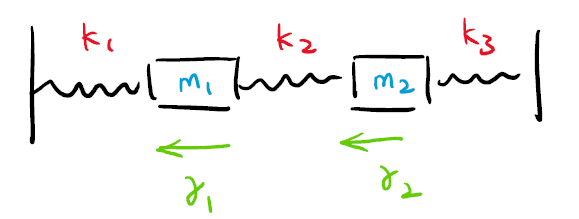
\includegraphics[width=\textwidth]{shm}
    \end{minipage}
\end{center}

In this configuration, let the displacement of mass 1 $=x_1(t)$,
displacement of mass 2 $=x_2(t)$.

\begin{itemize}
    \item \ul{Newton's \nth{2} Law for $m_1$}:\\[-2.5em]
    \begin{center}
        \begin{minipage}{0.4\linewidth}
            \centering
            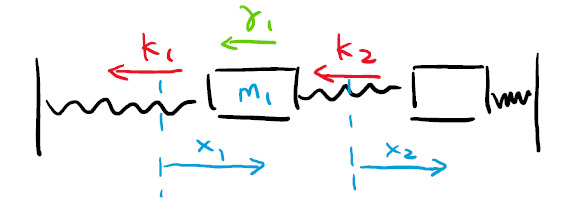
\includegraphics[width=\textwidth]{shm_m1}
        \end{minipage}
    \end{center}

    \begin{itemize}
        \item Left spring ($k_1$) change in length = $|x_1|$
        \item Right spring ($k_2$) change in length = $|x_2-x_1|$
    \end{itemize}
    \aleq{
        \therefore \ F = m_1\dvv[2]{t}x_1 = -k_1x_1-k_2(x_1-x_2)-\gamma_1 \dvv{t}x_1
    }

    \vskip 1ex
    \item \ul{Newton's \nth{2} Law for $m_2$}:\\[-2.5em]
    \begin{center}
        \begin{minipage}{0.4\linewidth}
            \centering
            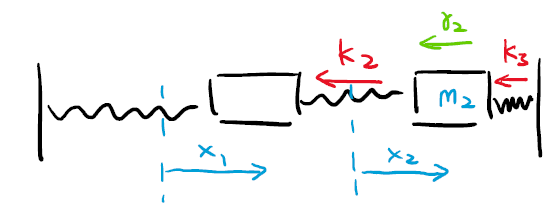
\includegraphics[width=\textwidth]{shm_m2}
        \end{minipage}
    \end{center}

    \begin{itemize}
        \item Left spring ($k_2$) change in length = $|x_2-x_1|$
        \item Right spring ($k_3$) change in length = $|x_2|$
    \end{itemize}
    \aleq{
        \therefore \ F = m_1\dvv[2]{t}x_2 = -k_3x_2-k_2(x_2-x_1)-\gamma_2 \dvv{t}x_2
    }
\end{itemize}

Group the 2 equations and transform it into a \nth{1} order system:
\aleq{
    \bcase{\barray{cccccc}{
        \dvv{t}u_1 &= &-\dfrac{\gamma_1}{m_1}u_1 & &-\dfrac{k_1+k_2}{m_1}x_1 &+ \dfrac{k_2}{m_1}x_2\\[1em] 
        \dvv{t}u_2 &= & &-\dfrac{\gamma_2}{m_2}u_2 &+\dfrac{k_2}{m_2}x_1 &-\dfrac{k_2+k_3}{m_2}x_2\\[1em]
        \dvv{t}x_1 &= &u_1 & & &\\[1em]
        \dvv{t}x_2 &= & &u_2 & &
    }}
}
\aleq{
    \Rightarrow \ \dvv{t}\bmat{u1\\u_2\\x_1\\x_2} = 
    \bmat{
        -\dfrac{\gamma_1}{m_1} & 0 & -\dfrac{k_1+k_2}{m_1} & \dfrac{k_2}{m_1} \\
        0 & -\dfrac{\gamma_2}{m_2} &\dfrac{k_2}{m_2} & -\dfrac{k_2+k_3}{m_2} \\
        1 & 0 & 0 & 0 \\
        0 & 1 & 0 & 0
    }\bmat{u_1\\u_2\\x_1\\x_2}
}

\begin{center}
    \red{(Absolutely not recommend to waste time on solving it)}
\end{center}


%%%%%%%%%%%%%%
\subsection{Special Case: Coupled Symmetric System without Damping}

Here we only look into the results of a simplified case:
\begin{center}
    \blue{Let $k_1=k_3$, $\gamma_1=\gamma_2 = 0$, $m_1=m_2$}
\end{center}

The the Newton's \nth{2} Law reduce to 
\aleq{
    \bcase{\barray{cccc}{
        \dvv[2]{t}x_1 &= &-\dfrac{k_1+k_2}{m}x_1 &+\dfrac{k_2}{m}x_2\\[1em]
        \dvv[2]{t}x_2 &= &+\dfrac{k_2}{m}x_1 &-\dfrac{k_1+k_2}{m}x_2
    }}
}
\aleq{
    \dvv[2]{t}\bmat{x_1\\x_2} = 
    \bmat{-\dfrac{k_1+k_2}{m} &\dfrac{k_2}{m} \\ \dfrac{k_2}{m} &-\dfrac{k_1+k_2}{m}}
    \bmat{x_1\\x_2}
}

We do not have to break it into 4 equations.
We can already subsitute $\bmat{x1\\x_2}=\bmat{k_1\\k_2}e^{\omega t}$:
\aleq{
    \cus[red]{\omega^2}{\displaystyle \lambda} 
    \cus[red]{\bmat{k_1\\k_2}}{\displaystyle \mmat{x}}
    \ccancel[blue]{e^{\omega t}} = 
    \cus[red]{\bmat{-\dfrac{k_1+k_2}{m} &\dfrac{k_2}{m} \\ \dfrac{k_2}{m} &-\dfrac{k_1+k_2}{m}}}{\displaystyle \mmat{A}}
    \cus[red]{\bmat{k_1\\k_2}}{\displaystyle \mmat{x}}
    \ccancel[blue]{e^{\omega t}}
}

which is an eigenvalue problem to a $2\times 2$ matrix, 
with eigenvalues $=\omega^2$.
On solving we can find
\aleq{
    \barray{c|cc}{
        \omega^2\  & \dfrac{k_1}{m} & -\dfrac{k_1+2k_2}{m} \\[1em]\hline\\[-1.2em] 
        \bmat{k_1\\k_2}\  & \bmat{1\\1} & \bmat{1 \\ -1}
    }
}

So the general solution is
\aleq{
    \bmat{x_1\\x_2} = C_1\bmat{1\\1}e^{i\sqrt{\frac{k_1}{m}}t}
        + C_2\bmat{1\\1}e^{-i\sqrt{\frac{k_1}{m}}t}
        + C_3\bmat{1\\-1}e^{i\sqrt{\frac{k_1+2k_2}{m}}t}
        + C_4\bmat{1\\-1}e^{-i\sqrt{\frac{k_1+2k_2}{m}}t}
}

\bf{\ul{Physical Interpretation}}\\

The general solution is a superposition of 2 kinds of vibration of their own frequencies.\\ 
(i.e. 2 modes of vibrations).

\begin{itemize}
    \item \ul{Angular frequency 1: $\sqrt{\frac{k_1}{m}}$}
    \aleq{
        \bmat{x_1\\x_2} &= C_1\bmat{1\\1}e^{i\sqrt{\frac{k_1}{m}}t}
        + C_2\bmat{1\\1}e^{-i\sqrt{\frac{k_1}{m}}t}
        %
        = \boxed{\bmat{1\\1} A_1\cos\qty(\sqrt{\frac{k_1}{m}}t + \phi_1)}
    }

    In this pattern of vibration, $x_1=x_2=A\cos\qty(\sqrt{\frac{k_1}{m}}t+\phi)$\\[-1em]
    \begin{center}
        \begin{minipage}{0.75\linewidth}
            \centering
            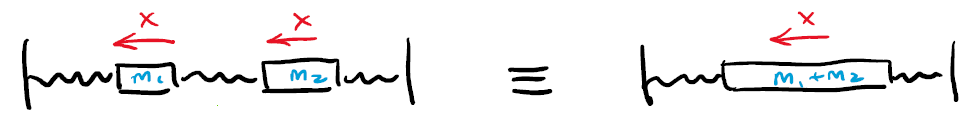
\includegraphics[width=\textwidth]{shm_inphase}
        \end{minipage}
    \end{center}

    $m_1,m_2$ always move together $\Rightarrow$ Call this the "in phase" mode.

    \item \ul{Angular frequency 2: $\sqrt{\frac{k_1+2k_2}{m}}$}
    \aleq{
        \bmat{x_1\\x_2} &= C_3\bmat{1\\-1}e^{i\sqrt{\frac{k_1+2k_2}{m}}t}
        + C_4\bmat{1\\-1}e^{-i\sqrt{\frac{k_1+2k_2}{m}}t}
        %
        =  \boxed{\bmat{1\\-1} A_2\cos\qty(\sqrt{\frac{k_1+2k_2}{m}}t + \phi_2)}
    }

    In this pattern of vibration, $x_1=-x_2=A\cos\qty(\sqrt{\frac{k_1+2k_2}{m}}t+\phi)$

    \begin{center}
        \begin{minipage}{0.8\linewidth}
            \centering
            
\includegraphics[width=\textwidth]{shm_outphase}
        \end{minipage}
    \end{center}

    $m_1,m_2$ always move in opposite direction $\Rightarrow$ Call this the "out of phase" mode.

\end{itemize}






%%%
\theend
\end{document}